\documentclass{article}

\usepackage[italian]{babel}
\usepackage[letterpaper,top=2cm,bottom=2cm,left=3cm,right=3cm,marginparwidth=1.75cm]{geometry}
\usepackage{amsmath}
\usepackage{graphicx}
\usepackage{subcaption}
\usepackage{textcomp}
\usepackage{float}
\usepackage{ragged2e}
\usepackage[dvipsnames]{xcolor}
\usepackage{fancyhdr}
\usepackage[colorlinks=true, allcolors=blue,
            pdfauthor={Matteo Drago},
            pdftitle={Casera Trentin},
            pdfsubject={Diario bivacchi e trekking},
            pdfkeywords={bivacco, montagna, trekking, diario}]{hyperref}
                
\title{\textbf{Casera Trentin - 1964 m s.l.m}}
\author{Matteo Drago}

% ==========================================================
% Impostazioni per il logo in ogni pagina
% ==========================================================
\pagestyle{fancy}
\fancyhf{} % Pulisce tutti i campi di intestazione e piè di pagina
\fancyhead[R]{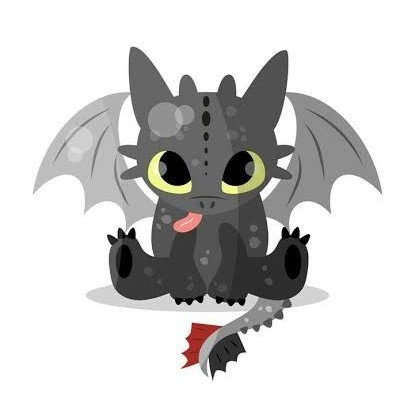
\includegraphics[height=1.5cm]{images/toothless.jpeg}} % Posiziona il logo a destra (R) nell'intestazione
\renewcommand{\headrulewidth}{0pt} % Rimuove la linea orizzontale nell'intestazione (opzionale)


\begin{document}
\maketitle
\thispagestyle{fancy} % Aggiungi questa riga

\begin{abstract}
Questo documento raccoglie e organizza le informazioni che ho acquisito nel corso degli anni sui bivacchi, basate sulle mie esperienze dirette. Sebbene non si proponga come una guida esaustiva e perfetta, offre il minimo indispensabile per una buona vita in bivacco, con consigli pratici e diretti per chiunque desideri affrontare al meglio queste pazze ma piacevoli avventure.
\end{abstract}

\section{Il bivacco}

% ==========================================================
% Immagine a sinistra, testo a destra allineato in alto
% ==========================================================
\noindent
\begin{minipage}[t]{0.45\textwidth}
  \vspace{0pt} % forza l'allineamento in alto
  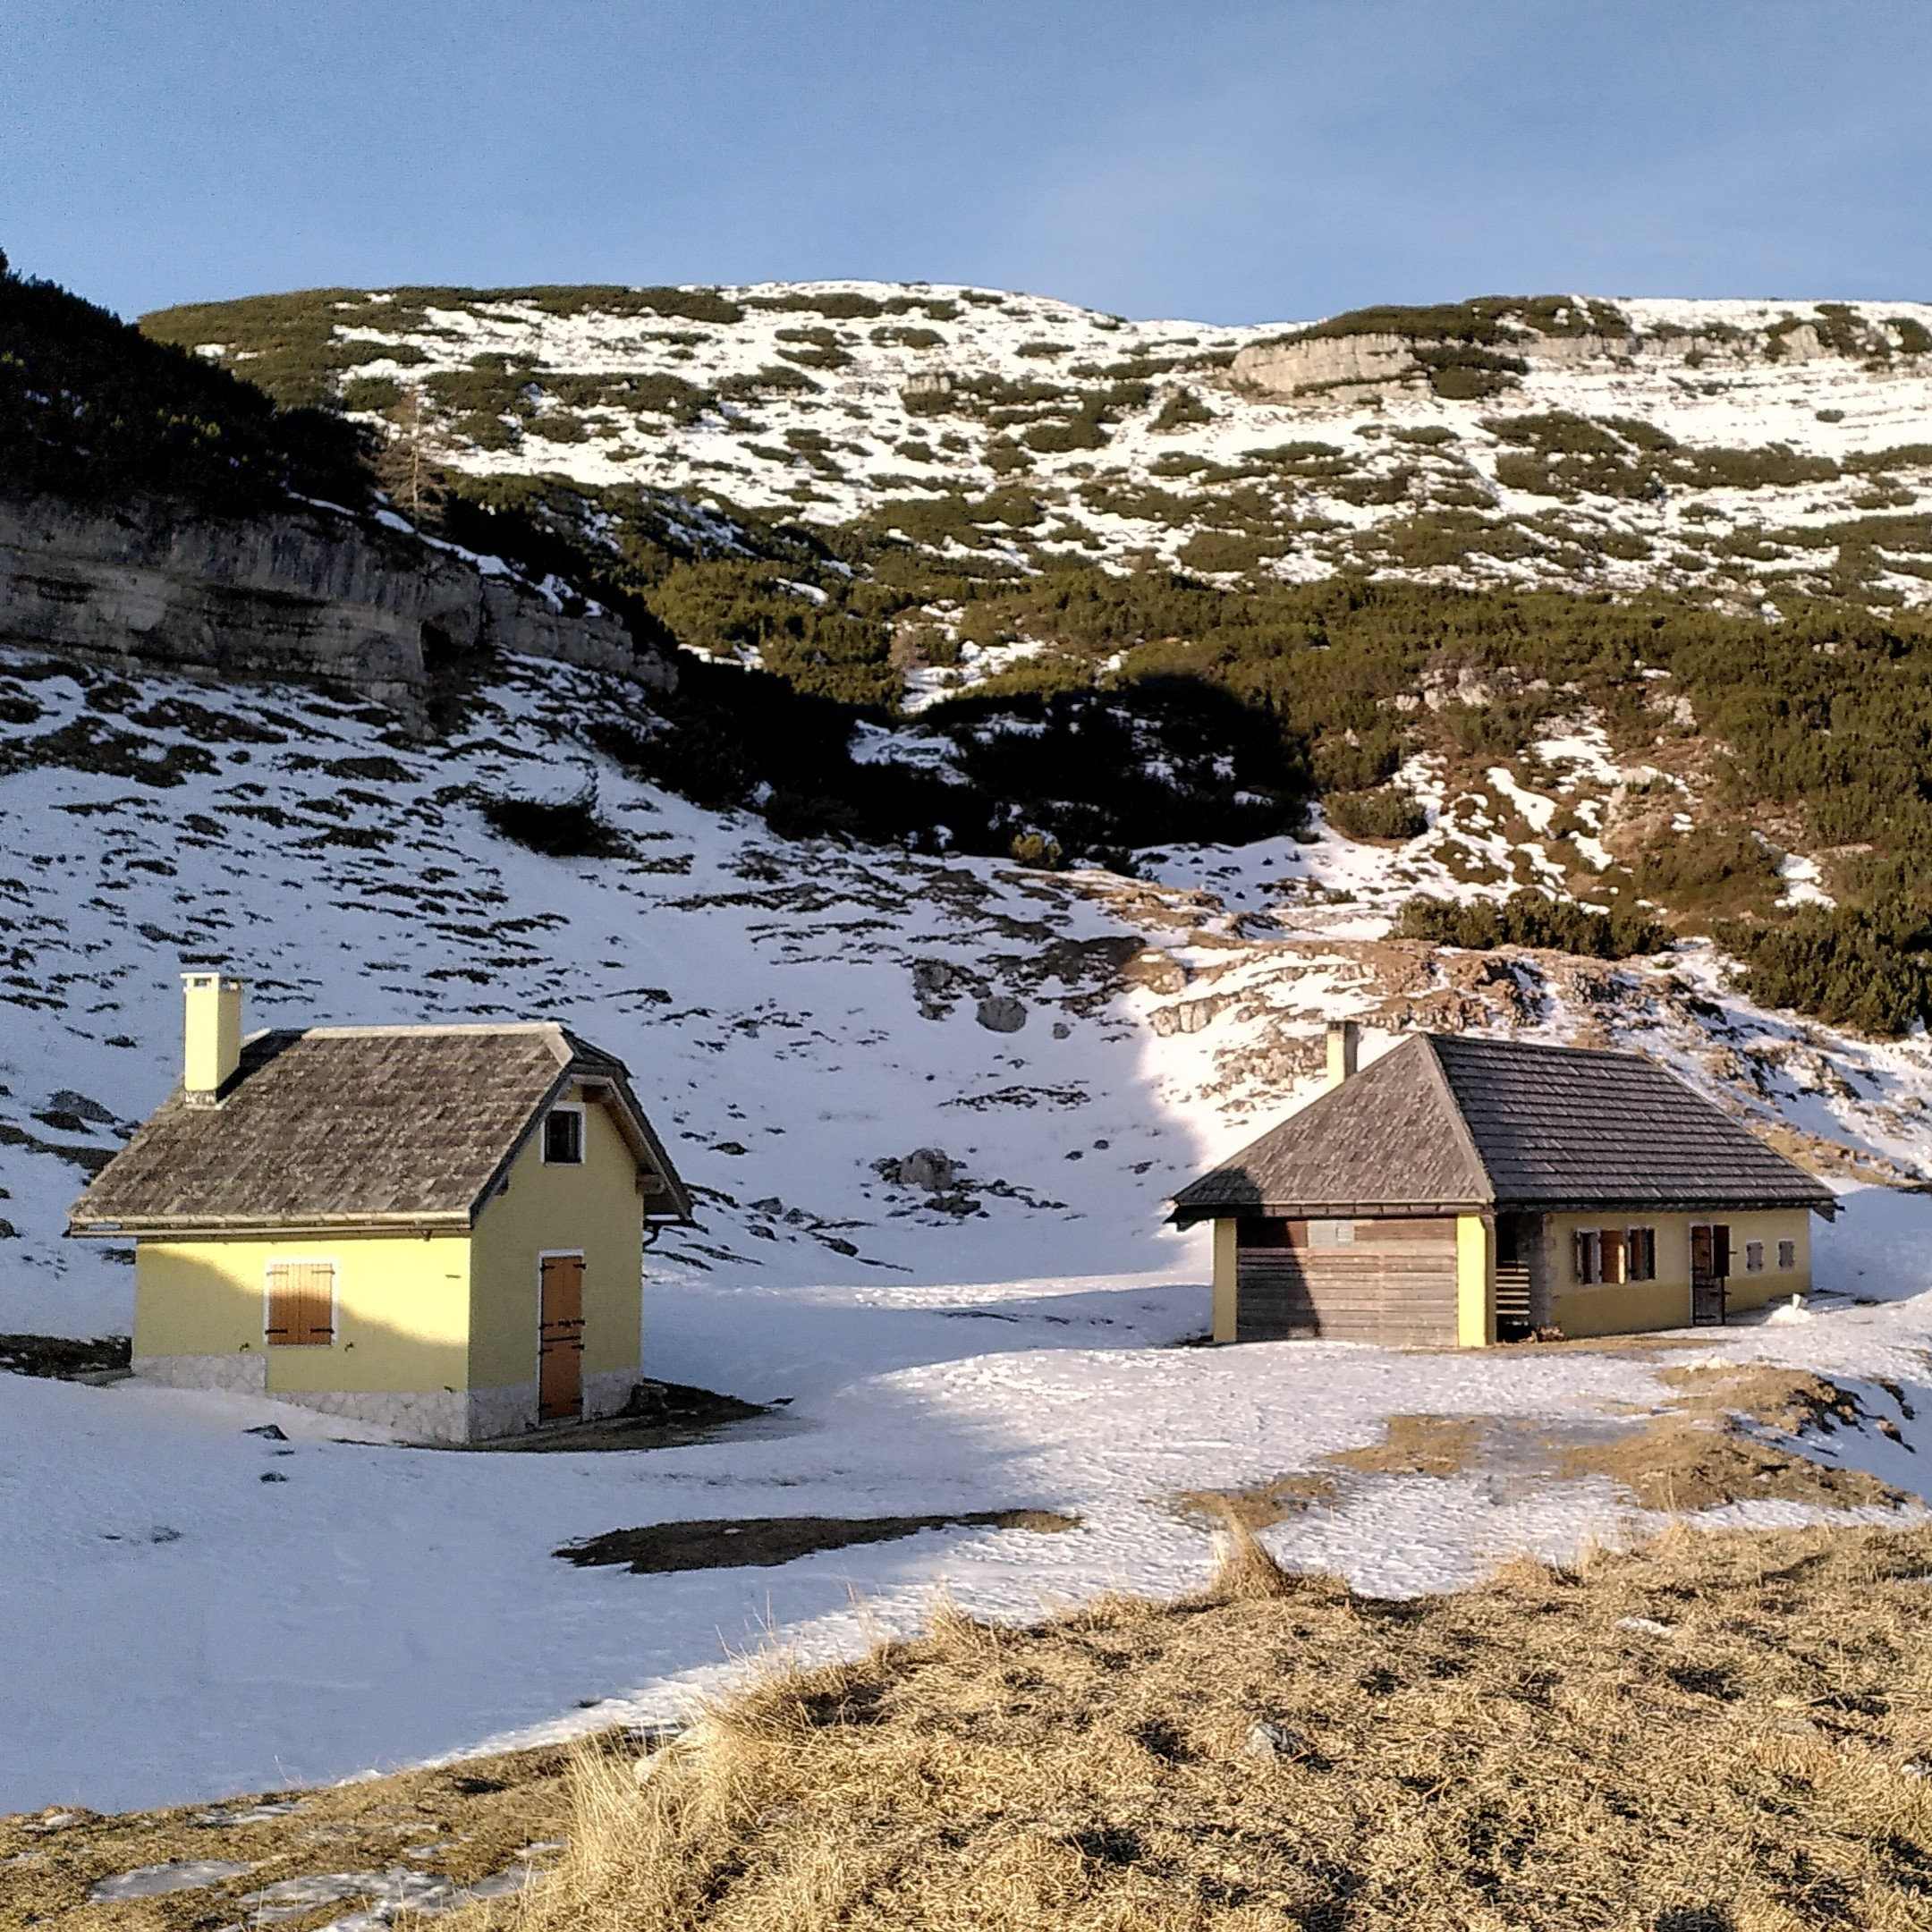
\includegraphics[width=\linewidth]{images/bivacco.jpg}
\end{minipage}%
\hfill
\begin{minipage}[t]{0.5\textwidth}
  \vspace{0pt} % forza l'allineamento in alto
  
  Gruppo montuoso\\
  \textbf{\large Altopiano dei 7 Comuni}
  \\[1em] % Aggiunge una riga vuota qui
  Località\\
  \textbf{\large Val Trentin}
  \\[1em] % Aggiunge una riga vuota qui
  Comune\\  
  \textbf{\large Asiago (VI)}
  \\[1em] % Aggiunge una riga vuota qui
  Altezza\\  
  \textbf{\large 1964 m s.l.m.}
  \\[1em] % Aggiunge una riga vuota qui
  Apertura\\  
  \textbf{\large Non gestito, sempre aperto}

\end{minipage}

\subsection{Caratteristiche}
Conosciuta anche come “Malga Portule Pastorile”, è la malga più alta dell’intero Altopiano. L’area circostante è in gran parte ricoperta da boschi di pino mugo e, durante il mese di agosto, la casèra viene utilizzata per poche settimane dai pastori.

Il bivacco è costituito da un’unica struttura sviluppata su più piani:
\begin{itemize}
    \item \textbf{Piano terra}: suddiviso in due stanze principali, di cui la più utilizzabile è quella con stufa, divano-letto, poltrona, camino e dispensa. La seconda stanza funge invece da magazzino per vecchi pezzi di stufa.
    \item \textbf{Piano superiore}: un soppalco accessibile tramite scala retrattile, con diverse brande distribuite su più locali, per un totale di circa 20 posti letto.
    \item \textbf{Spazio esterno}: ampio prato senza alberi da legna; tuttavia, il bivacco è dotato di una legnaia ben fornita.
\end{itemize}

Le stanze prive di stufa risultano molto fredde in inverno, a differenza della stanza principale che, grazie al camino e alla stufa, si mantiene calda e accogliente.

Nelle zone limitrofe al bivacco non sono presenti fonti d’acqua (dovrebbe esssercene una a circa 30 minuti di cammino, ma non siamo riusciti a trovarla), e ricavare legna non è facilissimo, data la predominanza di pino mugo.


\section{Come ci siamo arrivati}
Il bivacco è stato inserito in un giro di due giorni che comprendeva il Bivacco 3 Fontane e il Bivacco Casera Trentin.

Abbiamo parcheggiato l’auto al bivio di Basa Senocio (1100 m s.l.m.) e da lì ci siamo incamminati fino a raggiungere il Bivacco 3 Fontane. Il giorno successivo siamo ripartiti in direzione del Bivacco Casera Trentin, abbiamo raggiunto il Bivio Italia dove abbiamo pranzato ed esplorato il piccolo bivacco presente sulla cima per poi ripartire e raggiungere la Casera. Il giorno successivo siamo ripariti per ritornare al parcheggio.


\begin{figure}[htbp!]
    \centering
    % Colonna di sinistra, allineata in alto
    \begin{subfigure}[t]{0.45\textwidth}
        \centering
        \vspace{0pt} % Forziamo l'allineamento in alto
        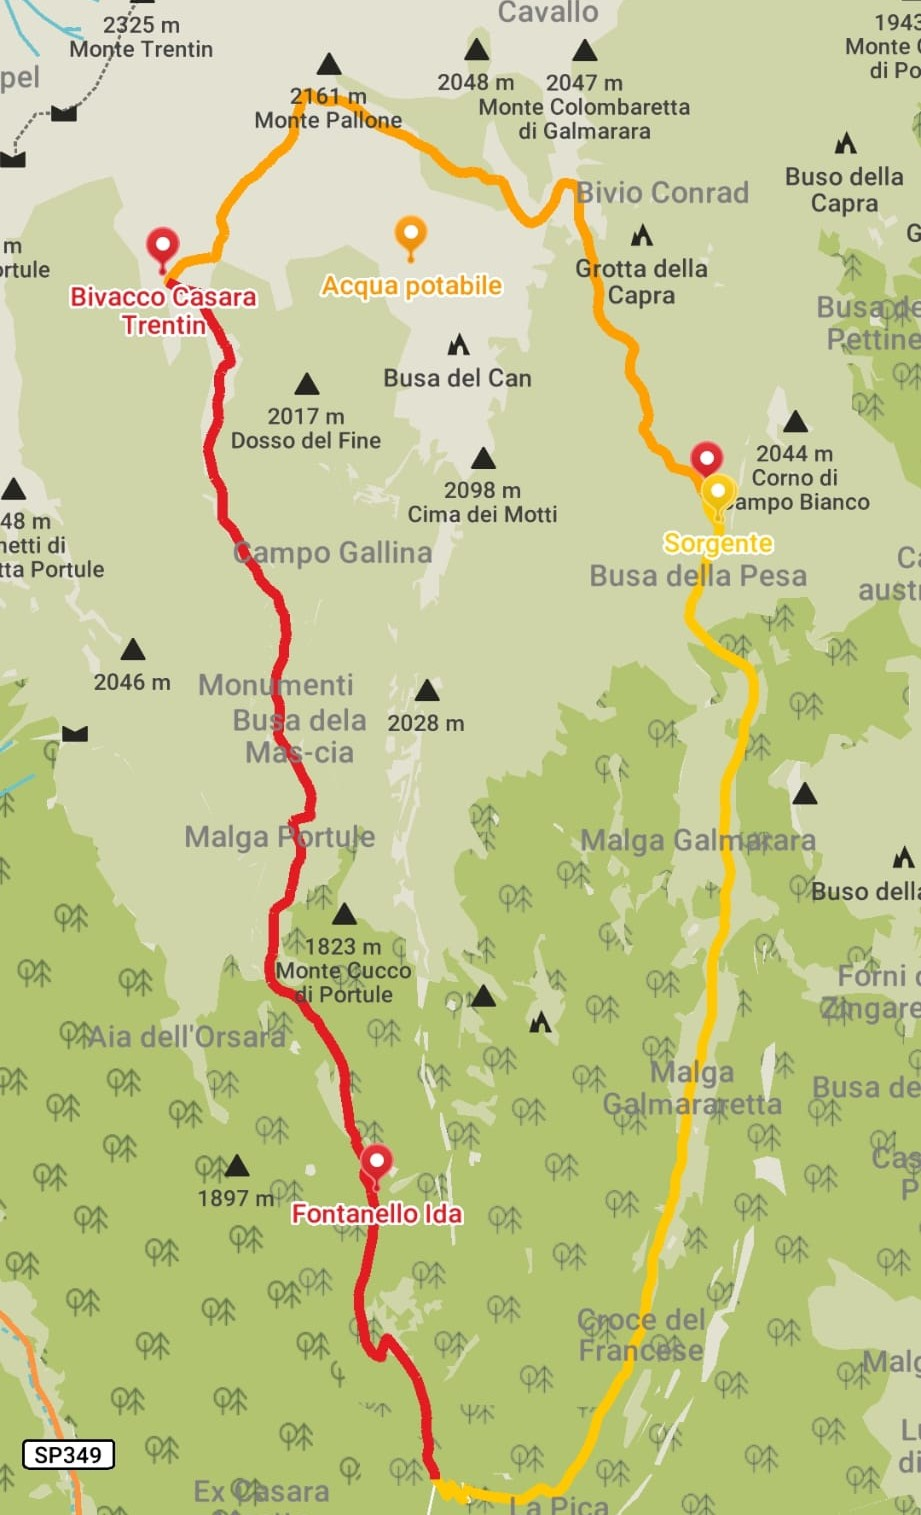
\includegraphics[width=\textwidth]{images/sentiero_mapsMe.jpg}
        \caption{Sentiero su Maps.Me.}
        \label{fig:foto_lunga}
    \end{subfigure}
    \hfill
    % Colonna di destra, allineata in alto
    \begin{subfigure}[t]{0.45\textwidth}
        \centering
        \vspace{0pt} % Forziamo l'allineamento in alto anche qui
        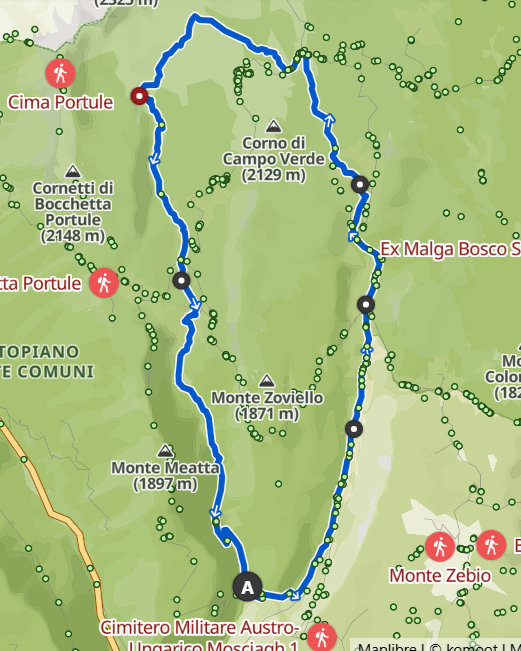
\includegraphics[width=\textwidth]{images/sentiero_komoot.png}
        \caption{Sentiero su Komoot.}
        \label{fig:foto_corta1}
        \vspace{1em} % Aggiunge un po' di spazio tra le due foto
        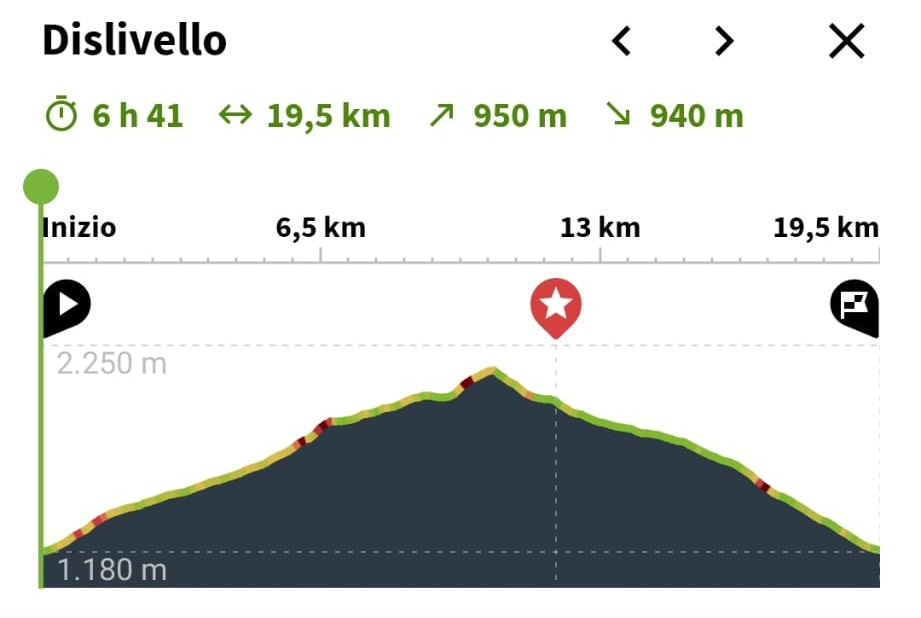
\includegraphics[width=\textwidth]{images/profilo_altimetrico.jpg}
        \caption{Profilo altimetrico del percorso.}
        \label{fig:foto_corta2}
    \end{subfigure}
    % Didascalia generale per l'intera figura
    \caption{Il sentiero e i dettagli del percorso.}
    \label{fig:panoramica_dettagli}
\end{figure}


\section{Non ti scordar di me}
\textbf{\textcolor{BurntOrange}{Ricorda: il bivacco è un bene comune. Il suo futuro dipende dal rispetto e dal senso civico dei visitatori. Usalo con cura e lascialo più pulito di come l'hai trovato.}}


\section{Esperienza personale}
Si è trattata di un'esperienza di 3 giorni con l'obiettivo di pernottare in 2 bivacchi, il 3 Fontane e la Casera Trentin. 
Siamo partiti dal bivacco 3 Fontane in direzione del Bivacco Casera Trentin, abbiamo raggiunto il Bivio Italia dove abbiamo pranzato ed esplorato il piccolo bivacco presente sulla cima per poi ripartire e raggiungere la Casera dopo aver superato un laghetto ghiacciato. La legna presente nella legnaia non era molta ma siamo comunque riusciti a riscaldare il bivacco per la notte. Il giorno successivo siamo ripartiti per ritornare al parcheggio. 


\section{Alcune foto}

% Sezione Alcune foto

\begin{figure}[htbp!]
    \centering
    % Prima riga: Due foto (QUESTA È LA PRIMA FIGURA)
    \begin{subfigure}[b]{0.45\textwidth}
        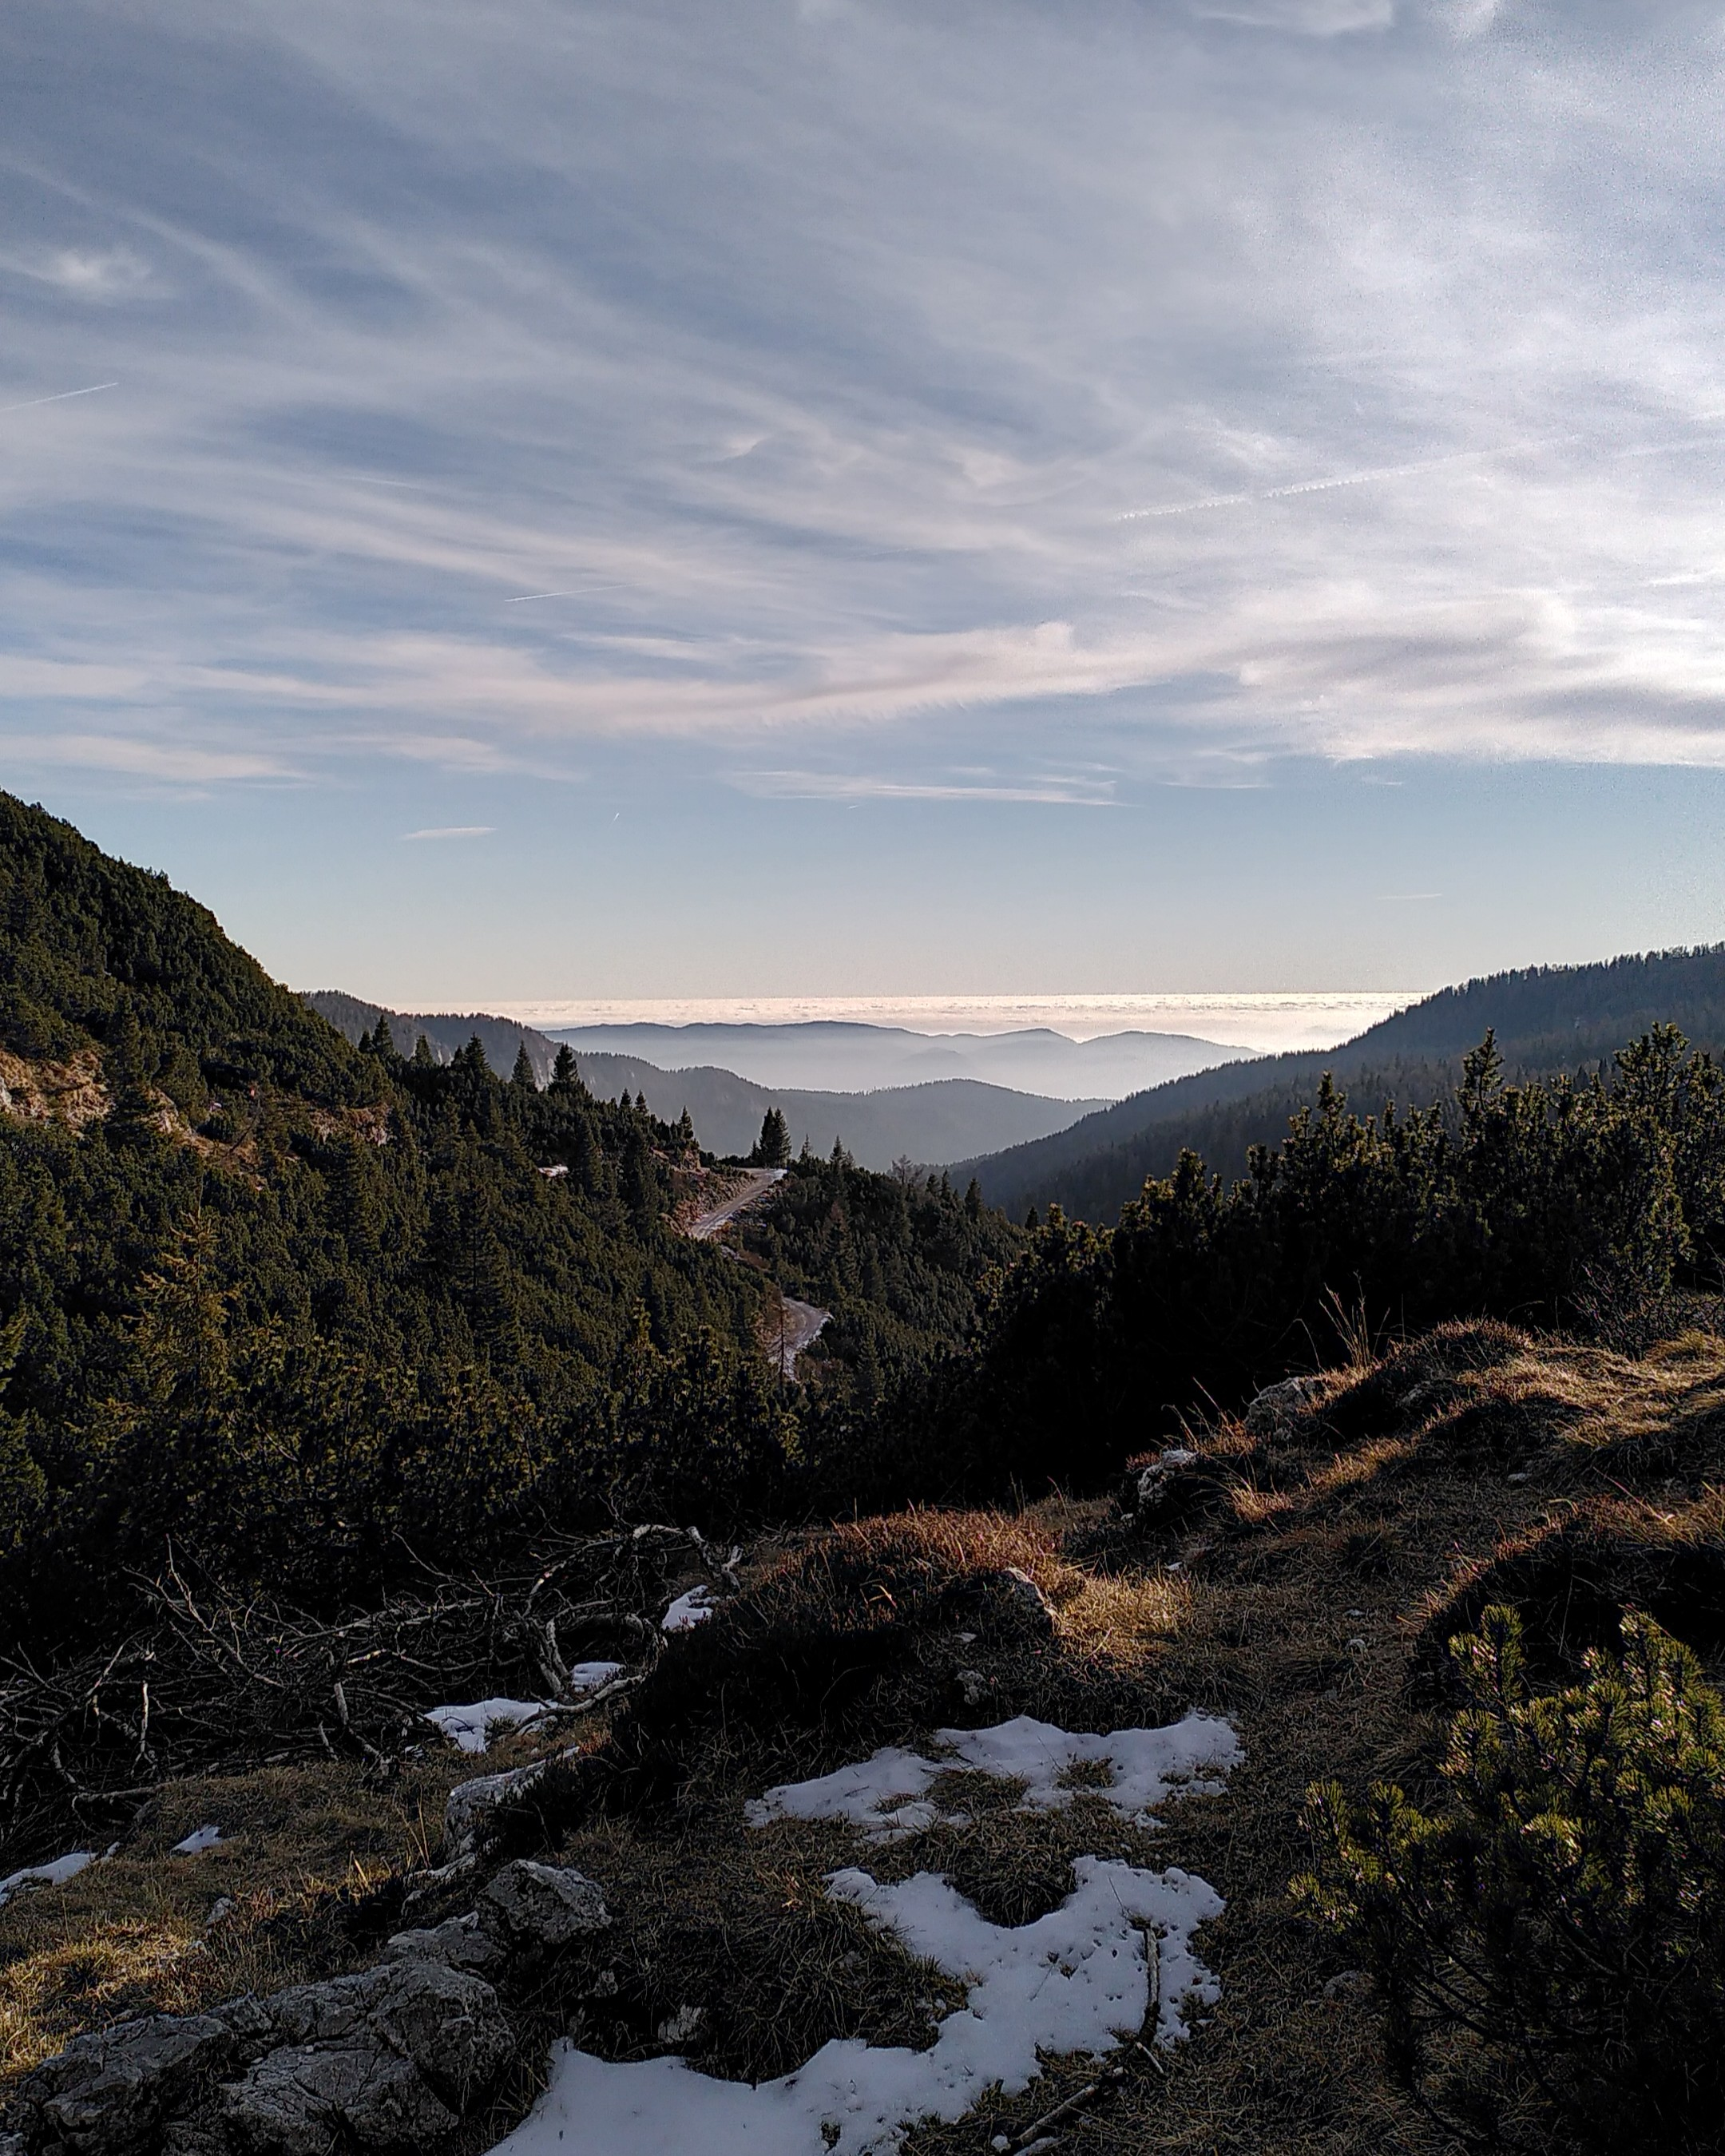
\includegraphics[width=\textwidth]{images/foto_sentiero.jpg}
        \caption{Sentiero.}
    \end{subfigure}
    \hfill
    \begin{subfigure}[b]{0.45\textwidth}
        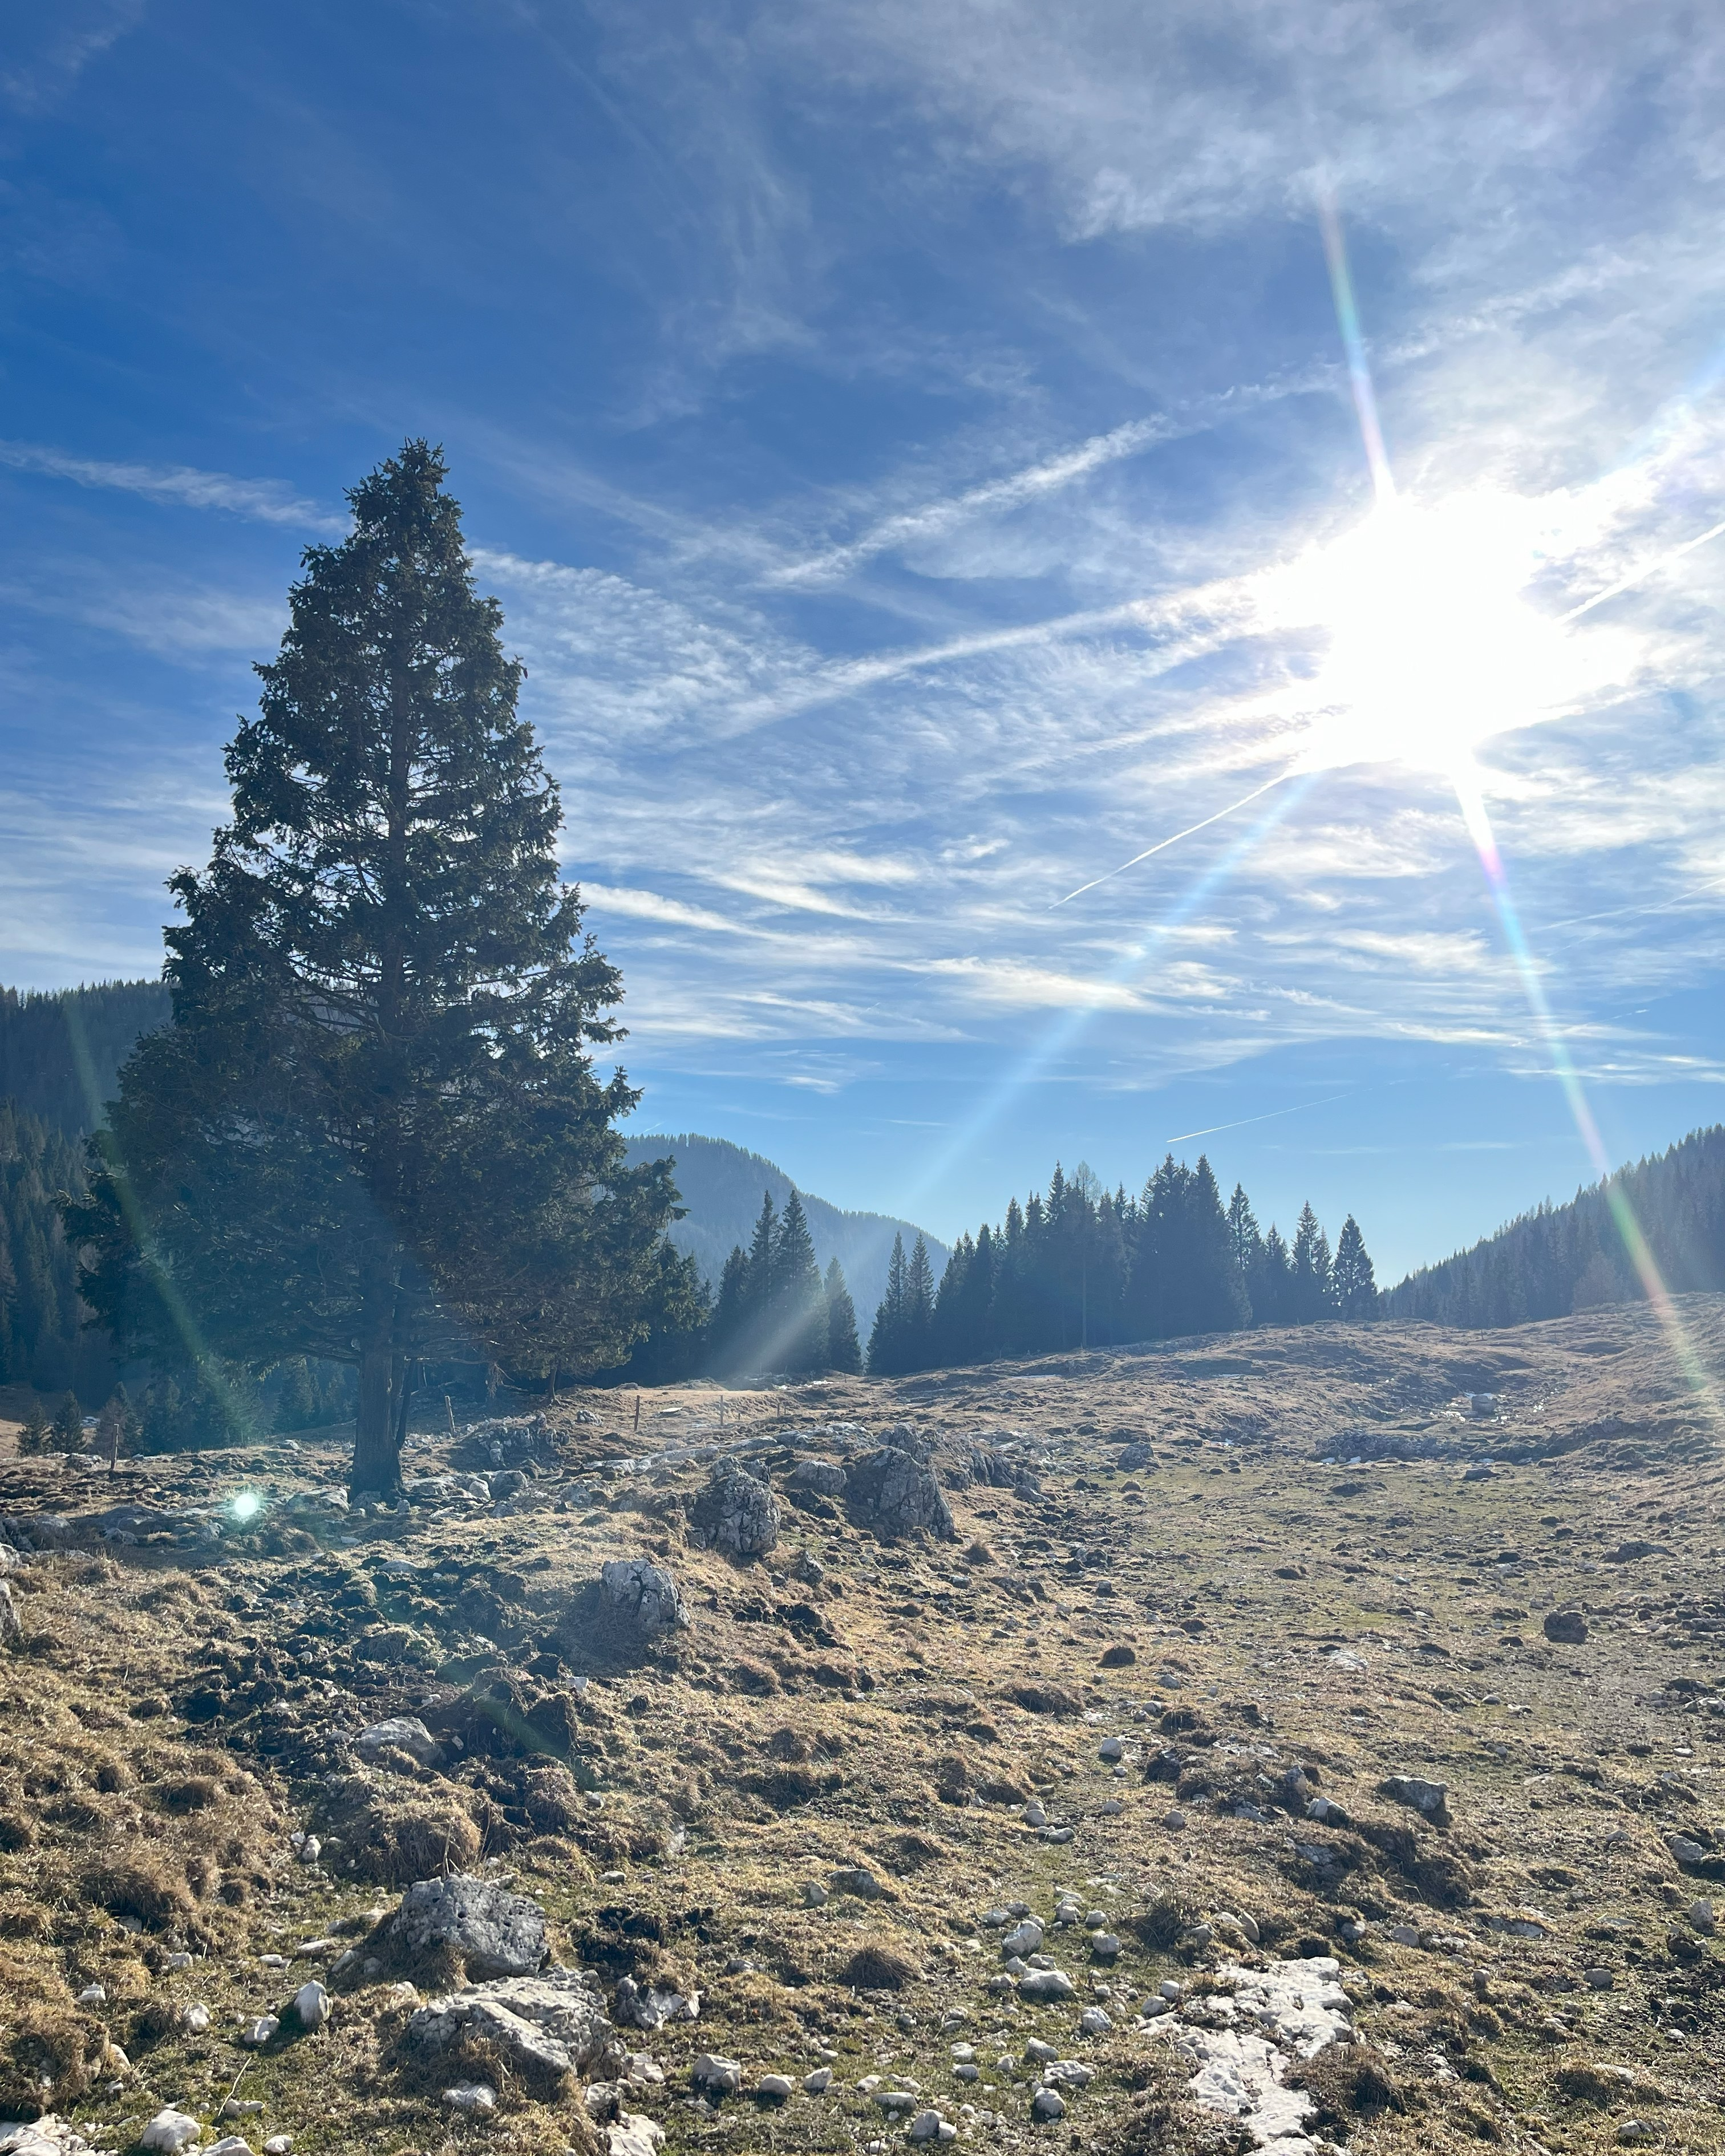
\includegraphics[width=\textwidth]{images/foto_paesaggio.jpg}
        \caption{Paesaggio.}
    \end{subfigure}

    \caption{Alcune foto.}
\end{figure}


\begin{figure}[H]
    \centering
    % Seconda riga: Tre foto (QUESTA È LA SECONDA FIGURA)
    \begin{subfigure}[b]{0.45\textwidth}
        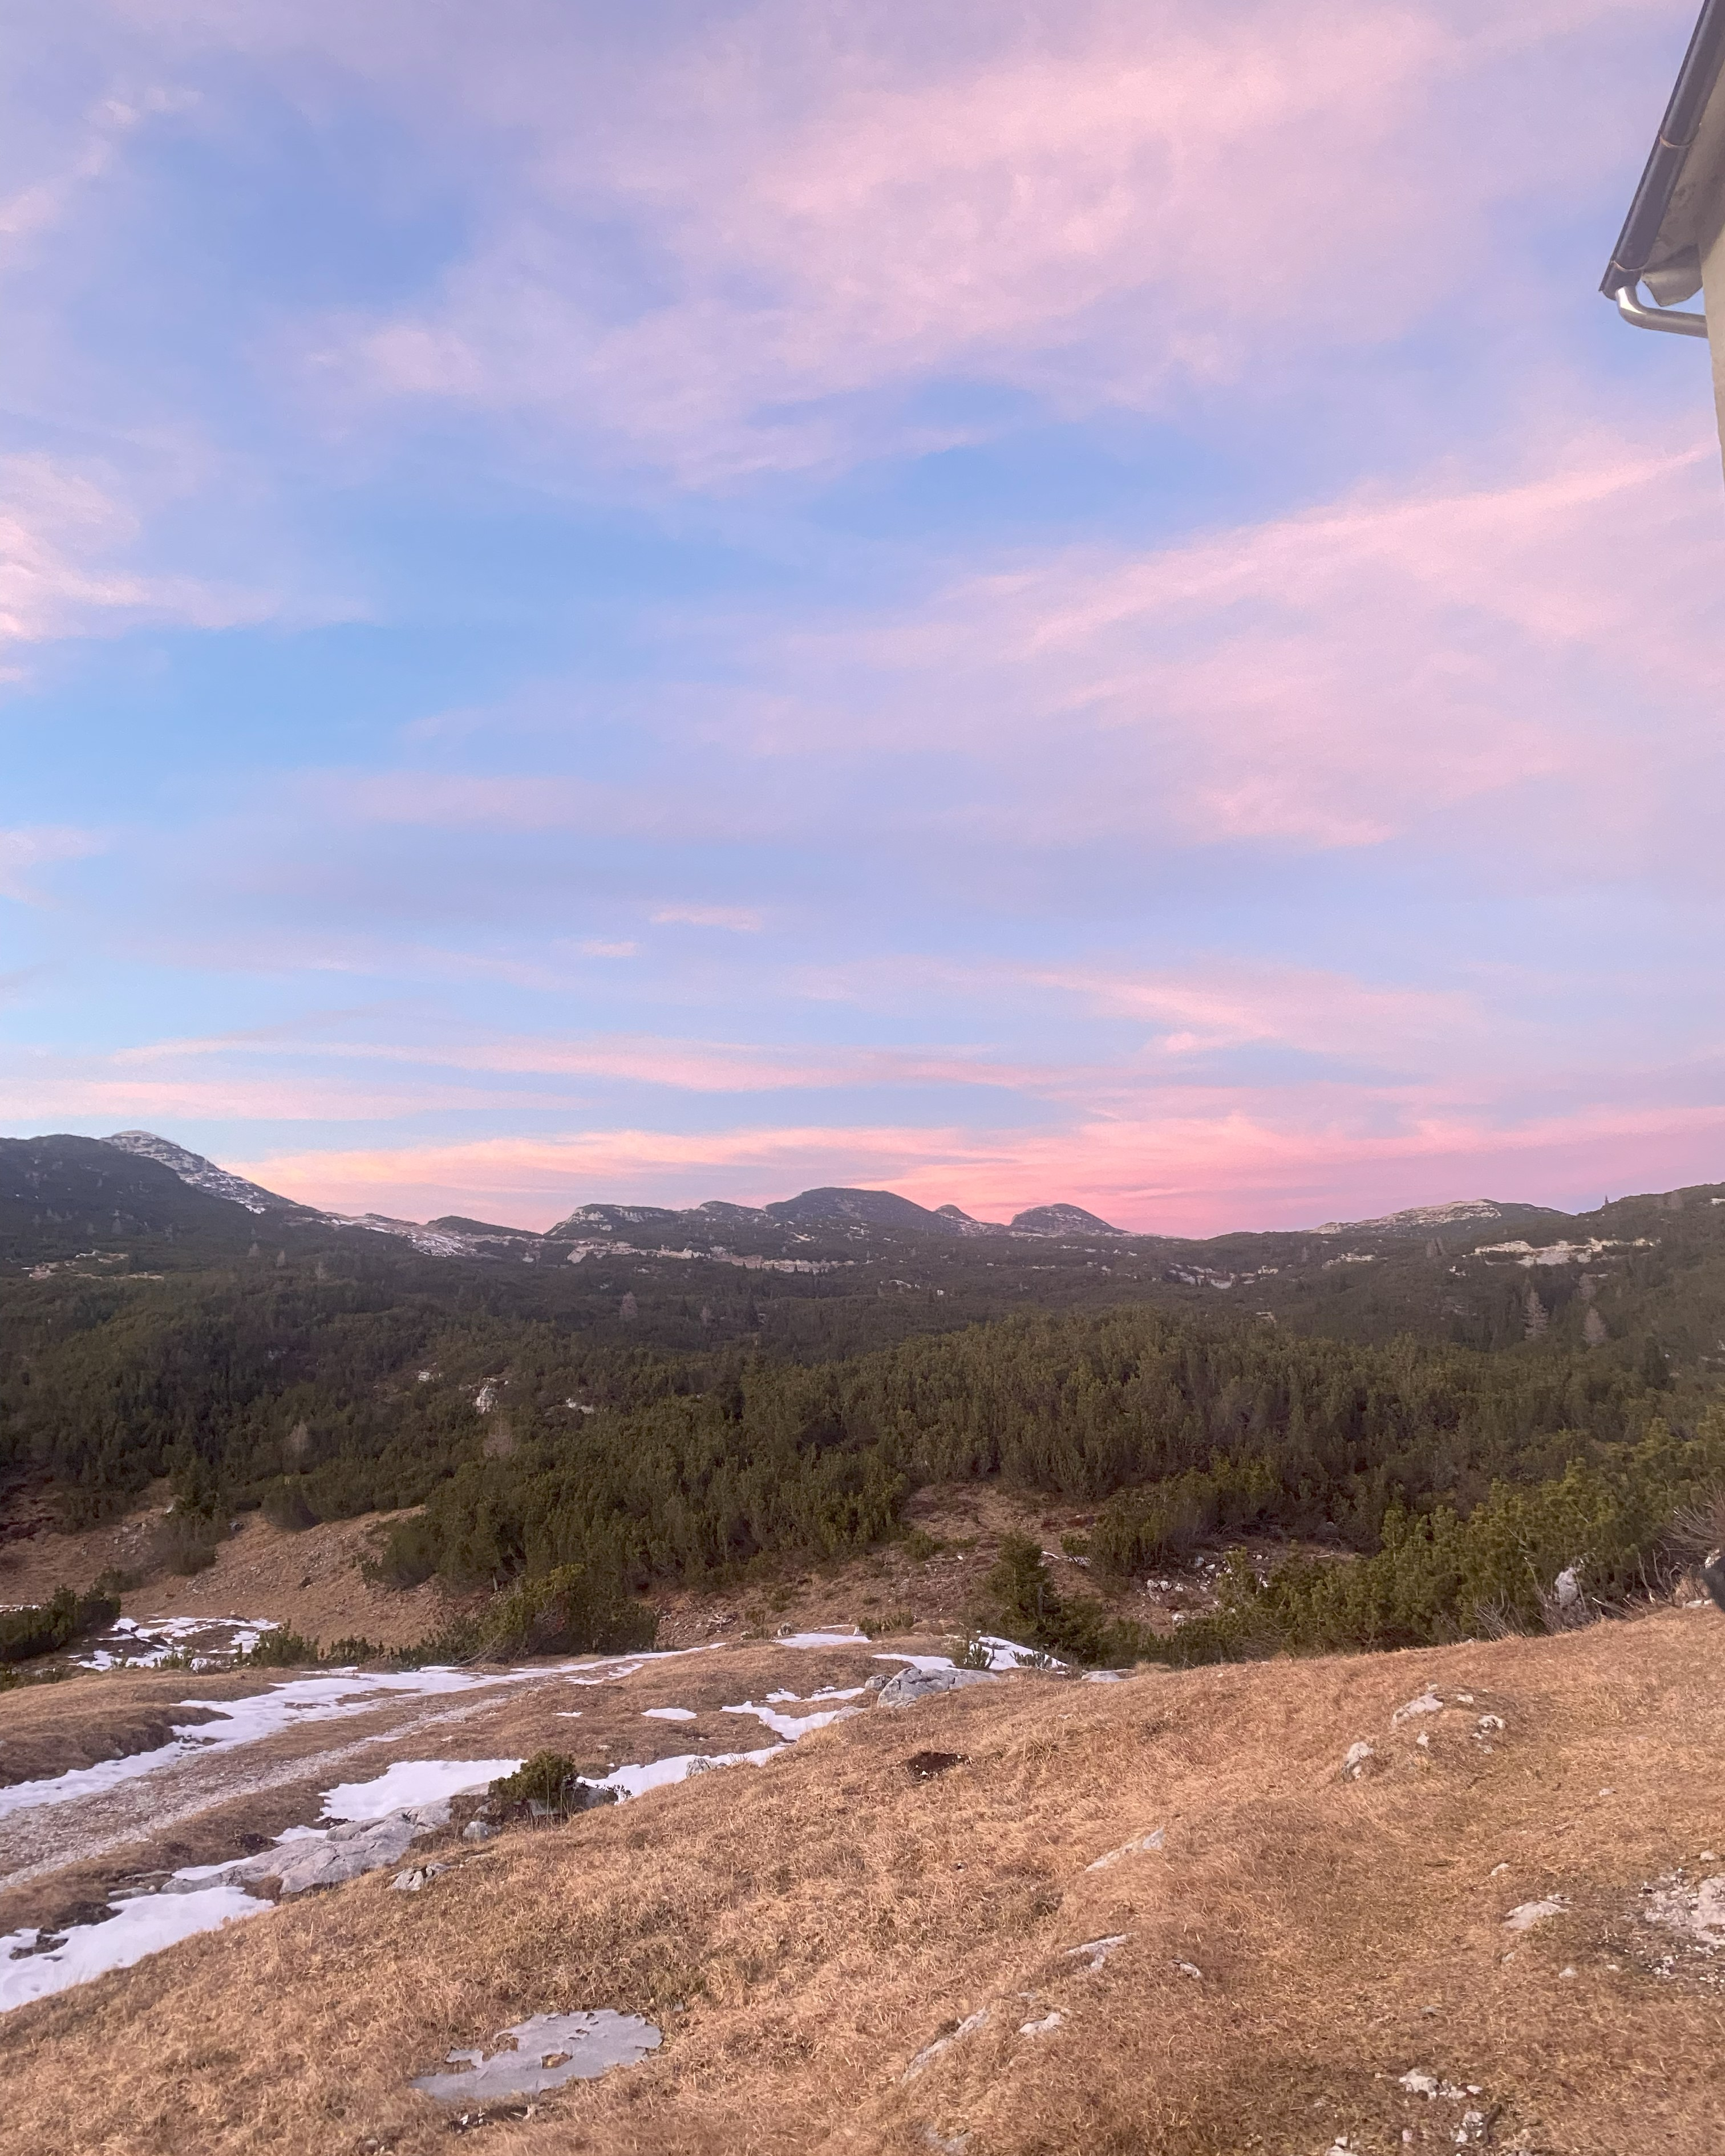
\includegraphics[width=\textwidth]{images/foto_bivacco.jpg}
        \caption{Altro paesaggio.}
    \end{subfigure}
    \hfill
    \begin{subfigure}[b]{0.45\textwidth}
        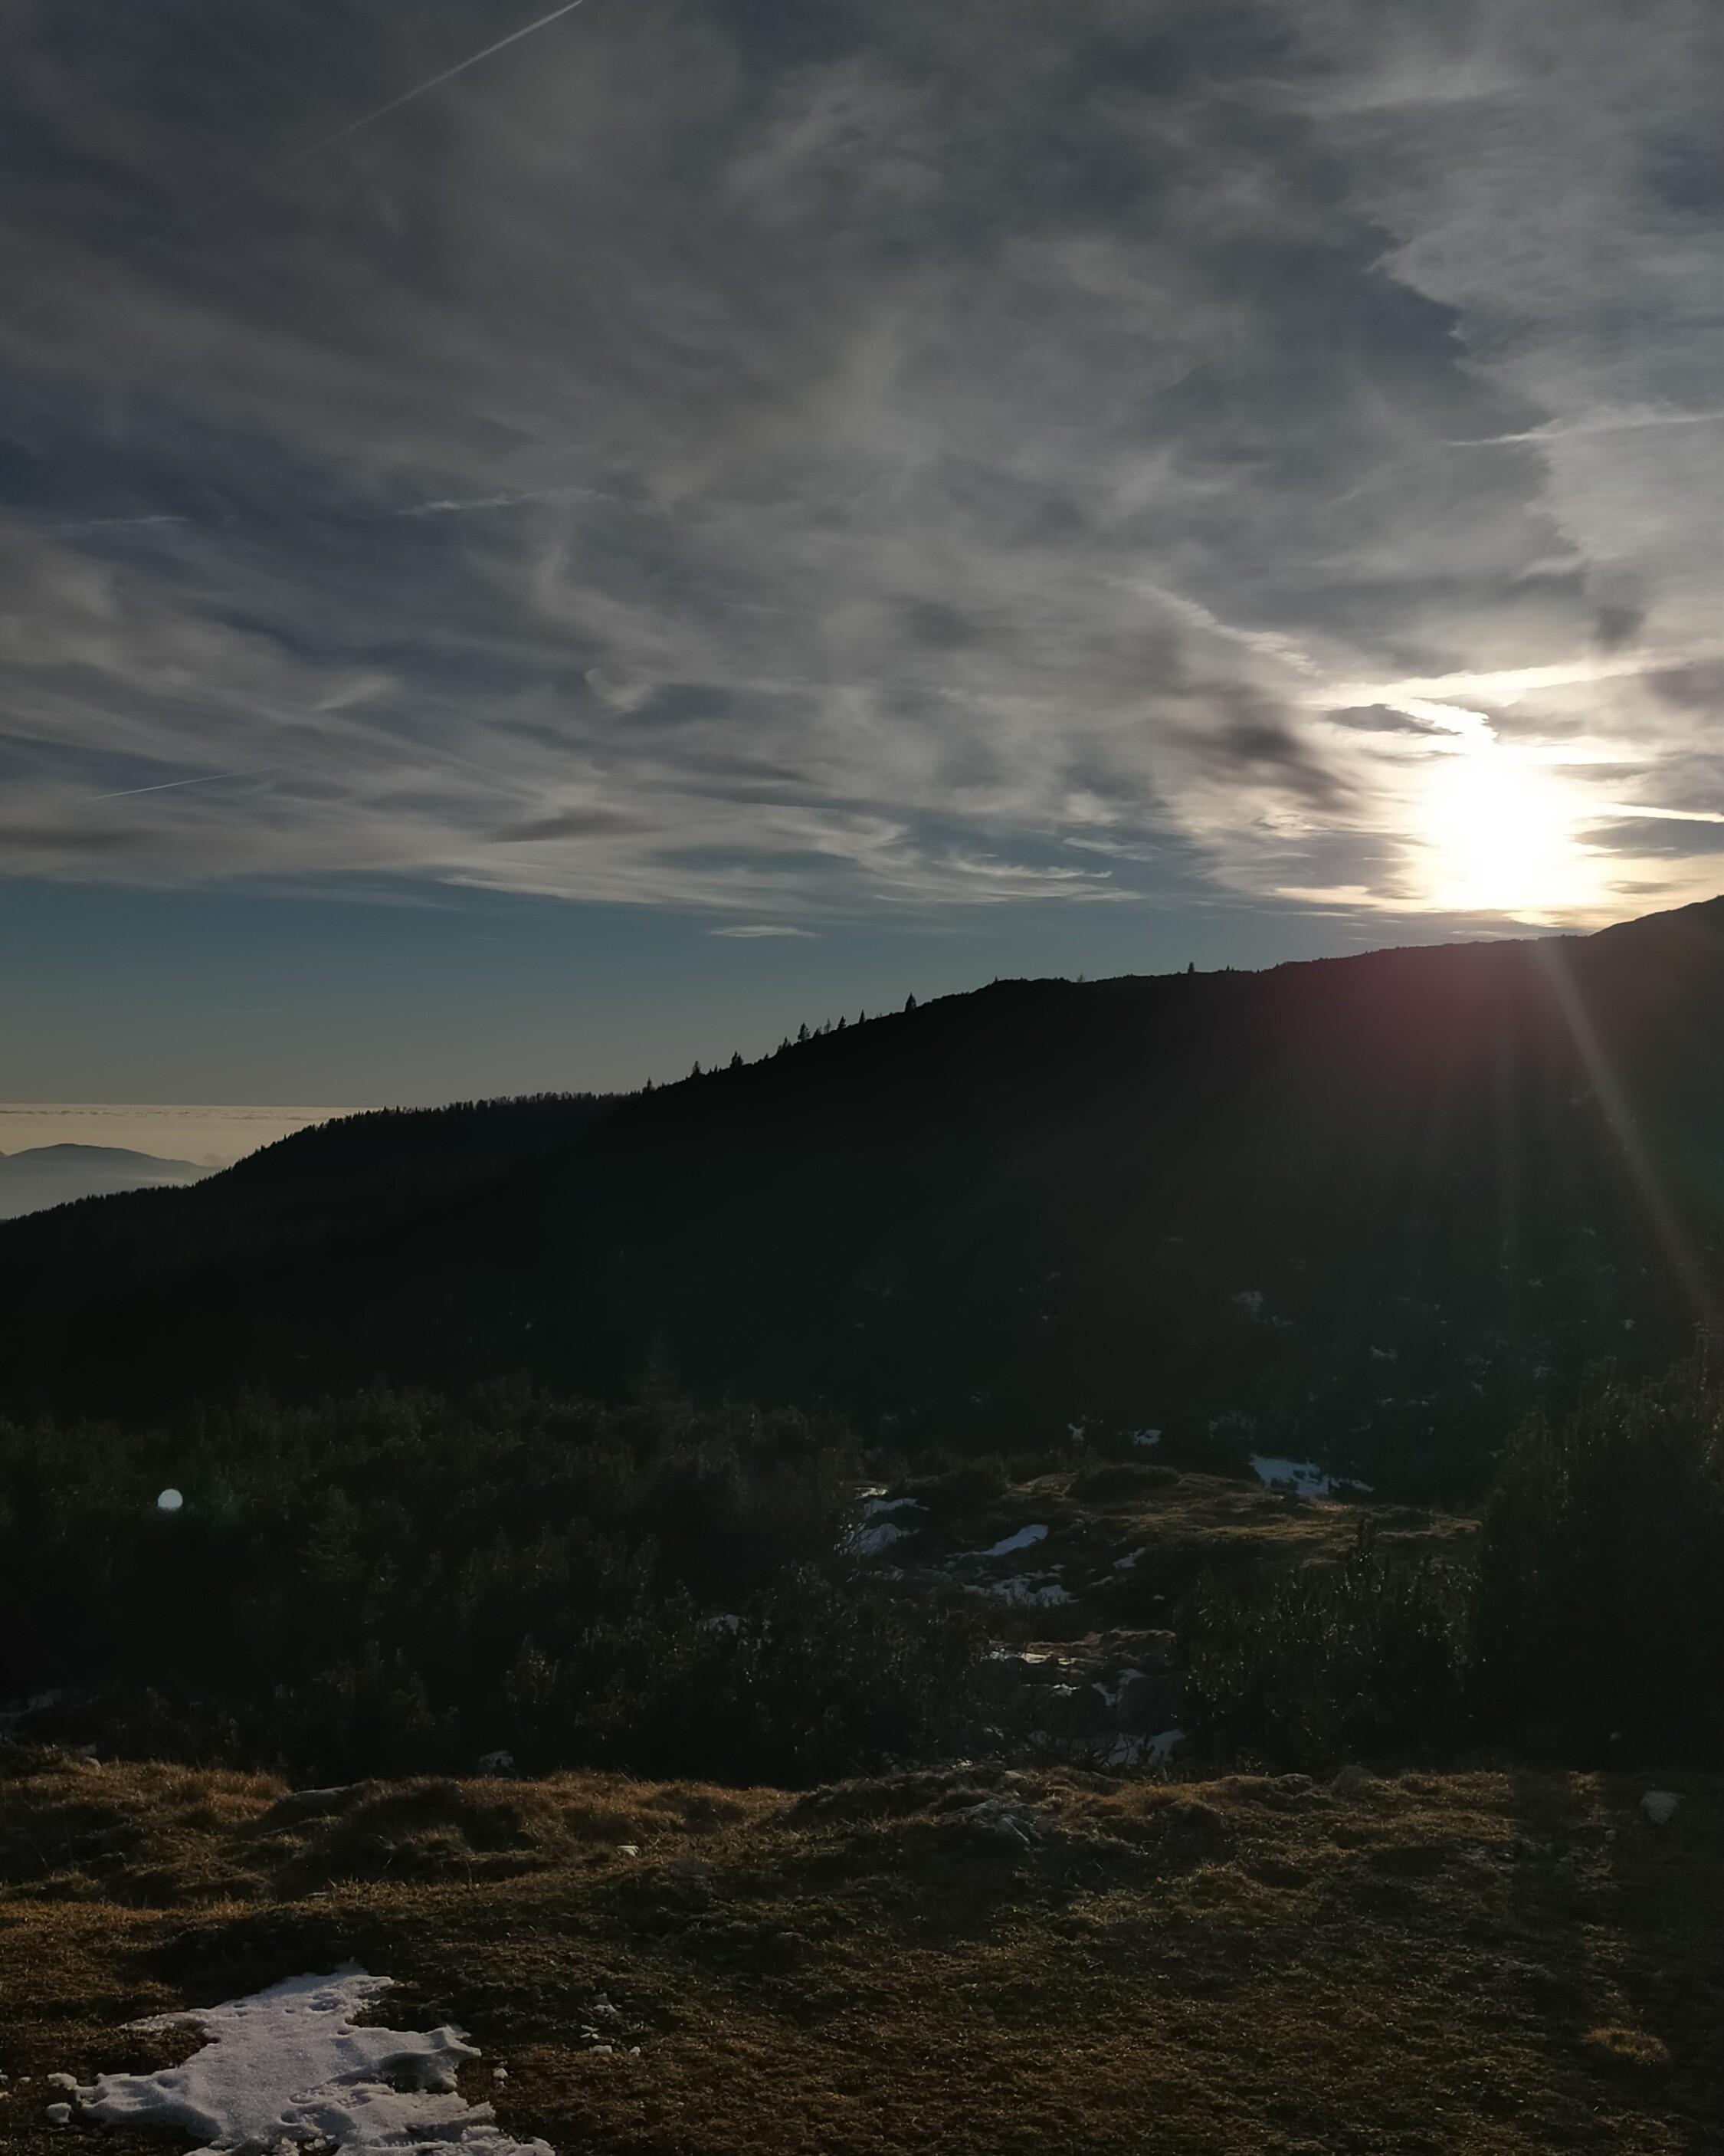
\includegraphics[width=\textwidth]{images/foto_tramonto.jpg}
        \caption{Vista al tramonto.}
    \end{subfigure}
    \hfill

    \caption{Selezione di fotografie del percorso e della vista dal bivacco.}
\end{figure}

\end{document}
